% arara: latex: { interaction: nonstopmode, options: ['-halt-on-error'] }
% arara: dvisvgm: { options: ['--no-fonts', '--exact-bbox', '--zoom=-1'] }
% From this directory: latex triangulation-11.tex
% dvisvgm --no-fonts --exact-bbox --zoom=-1 triangulation-11.dvi
\documentclass[tikz,border=4pt,11pt]{standalone}
\usetikzlibrary{arrows.meta}

\definecolor{ink}{HTML}{25313C}
\definecolor{voronoi}{HTML}{0072B2}
\definecolor{delaunay}{HTML}{C66A23}
\definecolor{cellone}{HTML}{E9EFFB}
\definecolor{celltwo}{HTML}{FDEDE4}
\definecolor{cellthree}{HTML}{E4F2EB}
\definecolor{cellfour}{HTML}{F0EAF7}
\definecolor{cellfive}{HTML}{FFF5D8}
\tikzset{
  primal/.style={draw=delaunay,line width=0.9pt,dash pattern=on 4pt off 3pt},
  dual/.style={draw=voronoi,line width=1.2pt},
  ray/.style={dual,-{Stealth[length=5pt,width=4pt]}},
  site label/.style={text=ink,inner sep=3pt},
  center label/.style={text=voronoi,inner sep=3pt},
}

\begin{document}
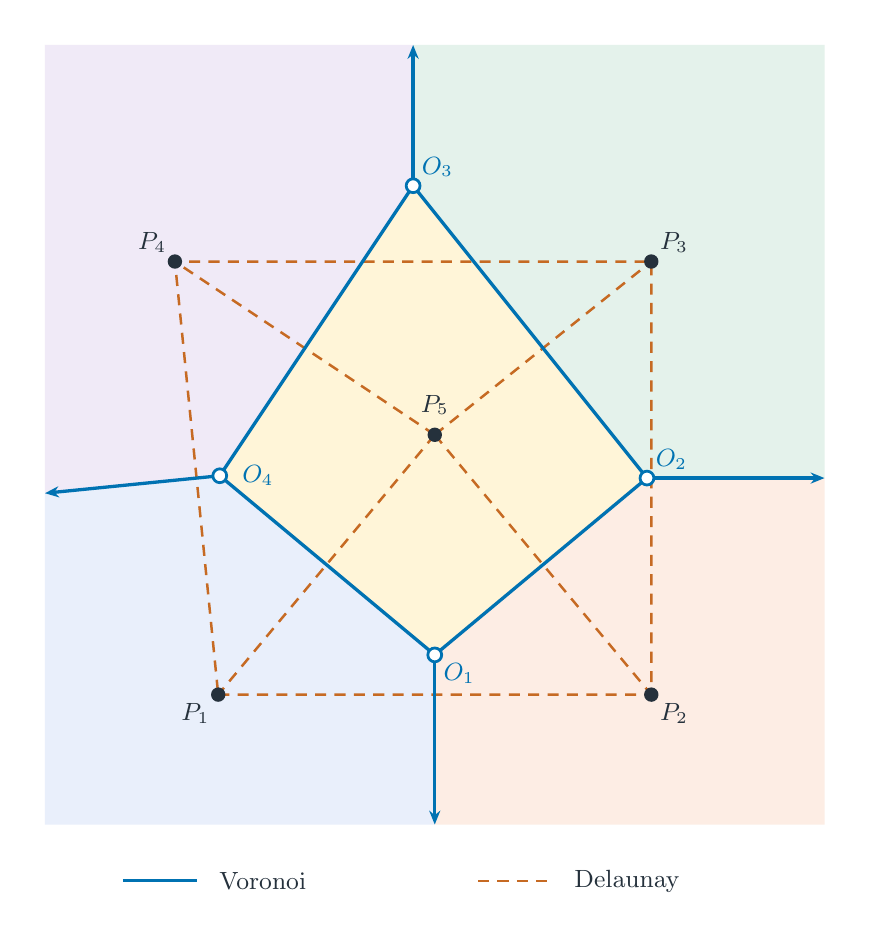
\begin{tikzpicture}[x=0.55cm,y=0.55cm,font=\small,text=ink]
  % A white margin and background keep the figure readable in dark themes.
  \fill[white] (-9.4,-10.2) rectangle (9.4,10.4);

  \coordinate (p1) at (-5,-5);
  \coordinate (p2) at (5,-5);
  \coordinate (p3) at (5,5);
  \coordinate (p4) at (-6,5);
  \coordinate (p5) at (0,1);

  % Circumcenters of (p5,p1,p2), (p5,p2,p3), (p5,p3,p4), (p5,p4,p1).
  % All other sites are strictly outside each corresponding circumcircle.
  \coordinate (o1) at (0,{-49/12});
  \coordinate (o2) at ({49/10},0);
  \coordinate (o3) at ({-1/2},{27/4});
  \coordinate (o4) at ({-139/28},{3/56});

  % Intersections of the unbounded Voronoi rays with the viewing window.
  % The ray directions are (0,-1), (1,0), (0,1), and (-10,-1).
  \coordinate (a) at (0,-8);
  \coordinate (b) at (9,0);
  \coordinate (c) at ({-1/2},10);
  \coordinate (d) at (-9,{-7/20});

  % Exact Voronoi cells clipped to [-9,9] x [-8,10].
  \fill[cellone] (-9,-8) -- (a) -- (o1) -- (o4) -- (d) -- cycle;
  \fill[celltwo] (a) -- (9,-8) -- (b) -- (o2) -- (o1) -- cycle;
  \fill[cellthree] (o2) -- (b) -- (9,10) -- (c) -- (o3) -- cycle;
  \fill[cellfour] (d) -- (o4) -- (o3) -- (c) -- (-9,10) -- cycle;
  \fill[cellfive] (o1) -- (o2) -- (o3) -- (o4) -- cycle;

  \draw[primal] (p1) -- (p2) -- (p3) -- (p4) -- cycle;
  \foreach \i in {1,...,4} {
    \draw[primal] (p5) -- (p\i);
  }

  \draw[dual] (o1) -- (o2) -- (o3) -- (o4) -- cycle;
  \draw[ray] (o1) -- (a);
  \draw[ray] (o2) -- (b);
  \draw[ray] (o3) -- (c);
  \draw[ray] (o4) -- (d);

  \foreach \i in {1,...,5} {
    \fill[ink] (p\i) circle[radius=2.6pt];
  }
  \node[site label,below left] at (p1) {$P_1$};
  \node[site label,below right] at (p2) {$P_2$};
  \node[site label,above right] at (p3) {$P_3$};
  \node[site label,above left] at (p4) {$P_4$};
  \node[site label,above=4pt] at (p5) {$P_5$};

  \foreach \i in {1,...,4} {
    \draw[voronoi,fill=white,line width=1pt] (o\i) circle[radius=2.5pt];
  }
  \node[center label,below right] at (o1) {$O_1$};
  \node[center label,above right] at (o2) {$O_2$};
  \node[center label,above right] at (o3) {$O_3$};
  \node[center label,right=5pt] at (o4) {$O_4$};

  \draw[dual] (-7.2,-9.3) -- (-5.5,-9.3);
  \node[anchor=west] at (-5.2,-9.3) {Voronoi};
  \draw[primal] (1,-9.3) -- (2.7,-9.3);
  \node[anchor=west] at (3,-9.3) {Delaunay};
\end{tikzpicture}
\end{document}
